\documentclass[dvisvgm]{standalone}
\usepackage{tikz}
\usetikzlibrary{shapes,arrows, positioning,fit}

\begin{document}
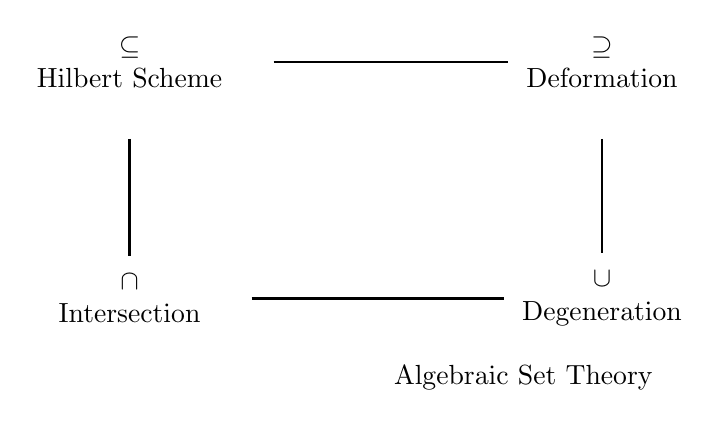
\begin{tikzpicture}[auto, every node/.style={align=center}]
  \node (a) at ( 0, 3) {$\subseteq$\\Hilbert Scheme};
  \node (b) at ( 6, 3) {$\supseteq$\\Deformation};
  \node (c) at ( 0, 0) {$\cap$\\Intersection};
  \node (d) at ( 6, 0) {$\cup$\\Degeneration};
  \draw[-, shorten <= 15pt, shorten >= 3pt, thick] (a)  -- (b);
  \draw[-, shorten <= 15pt, shorten >= 3pt, thick] (a)  -- (c);
  \draw[-, shorten <= 15pt, shorten >= 3pt, thick] (b)  -- (d);
  \draw[-, shorten <= 15pt, shorten >= 3pt, thick] (c)  -- (d);
  \node at ( 5, -1) {Algebraic Set Theory};
\end{tikzpicture}
\end{document}
